% Unit 121 English translation of chapter9.tex lines 1--305.
% Source: Methods of Algebra, Volume 2, commit
% 9a5803ff77dd3257484cb177f851a73770a59dd3 (CC BY 4.0).
% stable-unit-id: o014.aljabr2.chapter9.duality-a
% Coverage: the opening of Chapter 9 and Section 9.1 through the definition
% of dual morphisms; Unit 122 continues at line 306.

\hypertarget{o014.aljabr2.chapter9.duality-a}{ }
% segment-id: o014.aljabr2.chapter9.duality-a.h001
\chapter{Duality}\label{sec:duality}

% segment-id: o014.aljabr2.chapter9.duality-a.p001
The notion of duality originates in the theory of vector spaces. Let
$\Bbbk$ be a field, and denote the dual space of a $\Bbbk$-vector space $V$
by $V^\vee:=\Hom_{\Bbbk}(V,\Bbbk)$. There are
\begin{itemize}
	% segment-id: o014.aljabr2.chapter9.duality-a.i001
	\item the evaluation map $\mathrm{ev}:V\otimes V^\vee\to\Bbbk$, which
	sends $v\otimes\lambda$ to $\lambda(v)$;
	% segment-id: o014.aljabr2.chapter9.duality-a.i002
	\item if $V$ is finite-dimensional, also the coevaluation map
	$\mathrm{coev}:\Bbbk\to V^\vee\otimes V$, which sends $1$ to
	$\sum_{i=1}^n\check{v}_i\otimes v_i$, where $(v_i)_{i=1}^n$ is any basis
	of $V$ and $(\check{v}_i)_{i=1}^n$ its dual basis.
\end{itemize}

% segment-id: o014.aljabr2.chapter9.duality-a.p002
In the finite-dimensional case, they satisfy the fundamental identities
% segment-id: o014.aljabr2.chapter9.duality-a.q001
\[ (\identity_{V^\vee} \otimes \mathrm{ev})(\mathrm{coev} \otimes \identity_{V^\vee}) = \identity_{V^\vee}, \quad (\mathrm{ev} \otimes \identity_V) (\identity_V \otimes \mathrm{coev}) = \identity_V. \]

% segment-id: o014.aljabr2.chapter9.duality-a.p003
In a general monoidal category, the duality data defined in
\S\ref{sec:monoidal-dual} directly generalize the situation above: they
consist of a pair of objects $(L,R)$ together with morphisms
$\mathrm{ev}:L\otimes R\to\munit$ and
$\mathrm{coev}:\munit\to R\otimes L$ satisfying the preceding fundamental
identities. In this situation, $R$ is called a right dual of $L$, while $L$
is called a left dual of $R$. A monoidal category in which every object has
a left dual (respectively, a right dual) is called left rigid (respectively,
right rigid).

% segment-id: o014.aljabr2.chapter9.duality-a.p004
For braided monoidal categories, \S\ref{sec:symm-monoidal-dual} will explain
how the two kinds of dual are related. Thus, if an object $X$ has a dual, we
can define the trace $\Tr(f)$ of $f\in\End(X)$ and subsequently its dimension
$\dim X:=\Tr(\identity_X)$. Both are elements of $\End(\munit)$. Strictly
speaking, each has a left and a right version, but the two need not be
distinguished in a symmetric monoidal category. This book mainly discusses
abelian categories equipped with symmetric monoidal structures, such as
categories of modules over commutative rings (see
Proposition~\ref{prop:dualizable-module}). As long as the reader understands
the usefulness of dual vector spaces, the value of this generalization will
be self-evident. Duality becomes still more powerful in the setting of
$2$-categories, but that lies beyond the scope of this book.

% segment-id: o014.aljabr2.chapter9.duality-a.p005
Examples of duality are the subject of \S\ref{sec:duality-examples}. The
examples closest to algebra are the category
$\catesubd{Mod}{\mathrm{f}}A$ of finite-dimensional right $A$-modules for a
$\Bbbk$-Hopf algebra $A$, and its comodule counterpart
$\catesubd{Comod}{\mathrm{f}}A$ (Proposition~\ref{prop:Hopf-module-dual}).
In both cases, duality reflects properties of the antipode $S:A\to A$.
Examples involving Hopf algebras are important in the study of quantum
groups and also prepare the way for the theory of Tannakian categories.

% segment-id: o014.aljabr2.chapter9.duality-a.p006
The material in \S\S\ref{sec:coend}---\ref{sec:Hopf-reconstruction} of this
chapter concerns the coalgebra reconstruction problem. For every coalgebra
$L$, the abelian category $\catesubd{Comod}{\mathrm{f}}L$ is locally finite
(Definition~\ref{def:locally-finite}) and comes equipped with a faithful
exact forgetful functor
$U:\catesubd{Comod}{\mathrm{f}}L\to\cate{Vect}_{\mathrm{f}}(\Bbbk)$.
The reconstruction problem asks for a converse:
% segment-id: o014.aljabr2.chapter9.duality-a.b001
\begin{center}\begin{minipage}{0.8\textwidth}
	How can one construct a coalgebra $L$ from a locally finite
	$\Bbbk$-linear abelian category $\mathcal{A}$ and a faithful exact functor
	$\omega:\mathcal{A}\to\cate{Vect}_{\mathrm{f}}(\Bbbk)$ in such a way
	that $(\mathcal{A},\omega)$ is naturally equivalent to
	$(\catesubd{Comod}{\mathrm{f}}L,U)$?
\end{minipage}\end{center}
The approach taken in this chapter uses the coendomorphism coalgebra
$\coEnd(\omega)=\coEnd_{\Bbbk}(\omega)$ of the functor $\omega$
(Definition--Proposition~\ref{def:cogebra-L}). This coalgebra coacts on each
$\omega(X)$ and is ``universal'' with respect to these coactions.

% segment-id: o014.aljabr2.chapter9.duality-a.p007
The proof of the coalgebra reconstruction theorem,
Theorem~\ref{prop:Tannaka-aux1}, involves the theory of comonads from
\S\ref{sec:Beck}, basic Morita theory from \S\ref{sec:Morita}, a technical
result about locally finite abelian categories from
\S\ref{sec:locally-finite-Abel-cat}, and the Ind-ization introduced in
\S\ref{sec:Indization-functor}. If $(\mathcal{A},\omega)$ is equipped with
a monoidal structure, then $\coEnd(\omega)$ also becomes a bialgebra. If
$\mathcal{A}$ is both left and right rigid, then $\coEnd(\omega)$ is even a
Hopf algebra (Theorem~\ref{prop:Tannaka-aux2}). The presentation in this part
mainly follows \cite{Del90}.

% segment-id: o014.aljabr2.chapter9.duality-a.p008
After all these preparations, \S\ref{sec:Tannakian-cat} will introduce the
precise definition of a Tannakian category. These are symmetric monoidal
categories $\mathcal{T}$ with special properties. The formal definition is
due to N.\ Saavedra Rivano and P.\ Deligne, while its motivation goes back
to work of Tadao Tannaka and his successors. Among the conditions in
Definition~\ref{def:Tannakian-cat}, the most prominent is the existence of a
nonzero commutative $\Bbbk$-algebra $B$ and a right exact monoidal functor
$\omega:\mathcal{T}\to\cated{Mod}B$ compatible with the braiding; this is
called a fiber functor for $\mathcal{T}$ over $B$.

% segment-id: o014.aljabr2.chapter9.duality-a.p009
The setting of algebraic geometry requires that $B$ be allowed to be
general, but many elementary applications involve only neutral fiber
functors. In that case, $\omega$ is a faithful exact functor with values in
$\cate{Vect}_{\mathrm{f}}(\Bbbk)$. The corresponding neutral Tannakian
reconstruction theorem, Theorem~\ref{prop:Tannaka-neutral}, is simply an
application of the preceding results: it states that $\coEnd(\omega)$ is a
commutative Hopf algebra and identifies $(\mathcal{T},\omega)$ with
$(\catesubd{Comod}{\mathrm{f}}\coEnd(\omega),U)$.
\footnote{Translator's note: the source prints the second pair as
$(\coEnd(\omega),U)$. Since the first component of that pair must be a
category carrying the forgetful functor $U$, the well-typed expression is
$\catesubd{Comod}{\mathrm{f}}\coEnd(\omega)$.}
Many properties of $(\mathcal{T},\omega)$ are thereby translated into
properties of this Hopf algebra.

% segment-id: o014.aljabr2.chapter9.duality-a.p010
For a general fiber functor, Corollary~\ref{prop:Aut-Tannakian} relates the
commutative Hopf algebra $\coEnd_B(\omega)$ over $B$ to the group
$\Aut^\otimes(\omega)$ of $\otimes$-automorphisms of $\omega$. All the
information about $\coEnd_B(\omega)$ is contained in $\Aut^\otimes$, provided
the latter is understood as a group functor
$B\dcate{CAlg}\to\cate{Grp}$ rather than merely as a single group. This
viewpoint is entirely natural in algebraic geometry.

% segment-id: o014.aljabr2.chapter9.duality-a.p011
Finally, \S\ref{sec:TK} returns to the historical origins of Tannakian
categories. Using the preceding theory, it explains how to reconstruct a
finite group $G$ from the category $G\dcate{Mod}_{\mathrm{f}}$ of
finite-dimensional $G$-modules (Definition~\ref{def:G-mod}), together with
the forgetful functor $\omega$ to $\cate{Vect}_{\mathrm{f}}(\Bbbk)$. Since
in abstract harmonic analysis $G\dcate{Mod}_{\mathrm{f}}$ is in some sense a
``dual'' of $G$, this result is also called the finite-group version of the
Tannaka--Krein duality theorem. In fact, once it is known that $G$-modules
are the same as right comodules over the function space $C(G)$, the desired
isomorphism $G\rightiso\Aut^\otimes(\omega)$ has a shorter proof. The detour
through the reconstruction theorem is taken only to explain the origin of
Tannakian categories.

% segment-id: o014.aljabr2.chapter9.duality-a.rn001
\begin{wenxintishi}
	The sections on Hopf algebras, as well as the proof of the reconstruction
	theorem in \S\ref{sec:Tannaka-coend}, are based on some of the material in
	\CHref{sec:monads}. In addition, the proof of the reconstruction theorem
	uses \S\ref{sec:locally-finite-Abel-cat} and
	\S\ref{sec:Indization-functor} from the appendices; neither needs to be
	studied deeply on a first reading. The final section, \S\ref{sec:TK}, uses
	the basic notion of a $G$-module explained in the first half of
	\S\ref{sec:G-mod}; the discussion of resolutions in the second half of
	that section is not relevant to this chapter.
\end{wenxintishi}

% segment-id: o014.aljabr2.chapter9.duality-a.h002
\section{Duality in Monoidal Categories}\label{sec:monoidal-dual}

% segment-id: o014.aljabr2.chapter9.duality-a.p012
We first introduce a notion that applies to all monoidal categories and then
refine it step by step.

% segment-id: o014.aljabr2.chapter9.duality-a.d001
\begin{definition}\label{def:dualizable-obj}
	\index{dual}
	\index[sym1]{ev-coev}
	Let $\mathcal{C}$ be a monoidal category and
	$L,R\in\Obj(\mathcal{C})$. If there are morphisms
	% segment-id: o014.aljabr2.chapter9.duality-a.q002
	\[ \mathrm{ev}: L \otimes R \to \munit, \quad \mathrm{coev}: \munit \to R \otimes L \]
	such that the following two composites are $\identity_R$ and
	$\identity_L$, respectively, then $L$ is called a \emph{left dual} of
	$R$, while $R$ is called a \emph{right dual} of $L$:
	% segment-id: o014.aljabr2.chapter9.duality-a.q003
	\begin{gather*}
		R \simeq \munit \otimes R \xrightarrow{\mathrm{coev} \otimes \identity_R} (R \otimes L) \otimes R \simeq  R \otimes (L \otimes R) \xrightarrow{\identity_R \otimes \mathrm{ev}} R \otimes \munit \simeq R, \\
		L \simeq L \otimes \munit \xrightarrow{\identity_L \otimes \mathrm{coev}} L \otimes (R \otimes L) \simeq (L \otimes R) \otimes L \xrightarrow{\mathrm{ev} \otimes \identity_L} \munit \otimes L \simeq L.
	\end{gather*}
	The quadruple $(L,R,\mathrm{ev},\mathrm{coev})$ is called
	\emph{duality data}.
\end{definition}

% segment-id: o014.aljabr2.chapter9.duality-a.p013
The morphisms $\mathrm{ev}$ and $\mathrm{coev}$ in duality data should be
understood as ``evaluation'' and its dual. The unit constraints,
associativity constraints, and placement of parentheses involved in the
definition cause no difficulty and will often be suppressed from now on.

% segment-id: o014.aljabr2.chapter9.duality-a.p014
Definition~\ref{def:dualizable-obj} may remind the reader of the unit and
counit morphisms of adjoint functors. Duality does indeed encompass the
theory of adjoint functors, but to see this one must work in $2$-categories
or more general structures; that lies beyond the scope of this book.

% segment-id: o014.aljabr2.chapter9.duality-a.pr001
\begin{proposition}\label{prop:monoidal-functor-dual}
	Let $F:\mathcal{C}\to\mathcal{D}$ be a monoidal functor between monoidal
	categories. Every duality datum
	$(L,R,\mathrm{ev},\mathrm{coev})$ in $\mathcal{C}$ canonically induces
	the duality datum $(FL,FR,F\mathrm{ev},F\mathrm{coev})$ in $\mathcal{D}$.
\end{proposition}
% segment-id: o014.aljabr2.chapter9.duality-a.pf001
\begin{proof}
	To interpret $(FL,FR,F\mathrm{ev},F\mathrm{coev})$ as duality data, it
	suffices to consider the commutative diagram
	% segment-id: o014.aljabr2.chapter9.duality-a.g001
	\[\begin{tikzcd}
		FL \otimes FR \arrow[r] & \munit_{\mathcal{D}} \arrow[r] & FR \otimes FL \\
		F(L \otimes R) \arrow[r, "{F\mathrm{ev}}"'] \arrow[u, "\sim" sloped] & F(\munit_{\mathcal{C}}) \arrow[u, "\sim" sloped] \arrow[r, "{F\mathrm{coev}}"'] & F(R \otimes L) \arrow[u, "\sim"' sloped]
	\end{tikzcd}\]
	The vertical arrows come from the monoidal-functor structure. The required
	property is therefore reduced to the corresponding property in
	$\mathcal{C}$.
\end{proof}

% segment-id: o014.aljabr2.chapter9.duality-a.dp001
\begin{definition-proposition}\label{def:dual-uniqueness}
	\index[sym1]{Xstar@$X^*, {}^* X$}
	Let $\mathcal{C}$ be a monoidal category and
	$X\in\Obj(\mathcal{C})$. If $X$ has a right dual (respectively, a left
	dual), write its duality data as
	$(X,X^*,\mathrm{ev},\mathrm{coev})$ (respectively,
	$({}^*X,X,\mathrm{ev},\mathrm{coev})$). Then these data are unique up to
	unique isomorphism.

	Thus, without ambiguity, we may speak of the right dual $X^*$
	(respectively, the left dual ${}^*X$) of $X$.
\end{definition-proposition}
% segment-id: o014.aljabr2.chapter9.duality-a.pf002
\begin{proof}
	Reversing the order of $\otimes$ turns left duals into right duals and
	vice versa, so it suffices to treat the case of $X^*$. Suppose that the
	data $(X_i^*,\mathrm{ev}_i,\mathrm{coev}_i)$ give right duals of $X$, for
	$i=1,2$. First we prove uniqueness of the isomorphism. If
	$\alpha:X_1^*\rightiso X_2^*$ is compatible with the duality morphisms
	$\mathrm{ev}_i$ and $\mathrm{coev}_i$, then the following diagram
	commutes:
	% segment-id: o014.aljabr2.chapter9.duality-a.g002
	\[\begin{tikzcd}[row sep=tiny]
		X_1^* \arrow[dd, "\alpha"'] \arrow[r, "{\mathrm{coev}_2 \otimes \identity}" inner sep=0.6em] & X_2^* \otimes X \otimes X_1^* \arrow[dd, "{\identity \otimes \alpha}"] \arrow[rd, "{\identity \otimes \mathrm{ev}_1}"] & \\
		& & X_2^* \\
		X_2^* \arrow[r, "{\mathrm{coev}_2 \otimes \identity}"' inner sep=0.6em] & X_2^* \otimes X \otimes X_2^* \arrow[ru, "{\identity \otimes \mathrm{ev}_2}"'] &
	\end{tikzcd}\]
	By the definition of a right dual, the composite along the lower path is
	$(\identity\otimes\mathrm{ev}_2)(\mathrm{coev}_2\otimes\identity)
	=\identity_{X_2^*}$. The corresponding statement also holds for the
	inverse morphism $\beta:X_2^*\rightiso X_1^*$. Hence the desired
	morphisms $\alpha:X_1^*\to X_2^*$ and $\beta:X_2^*\to X_1^*$ can only be
	the composites
	% segment-id: o014.aljabr2.chapter9.duality-a.q004
	\begin{gather*}
		X_1^* \xrightarrow{\mathrm{coev}_2 \otimes \identity_{X_1^*}} X_2^* \otimes X \otimes X_1^* \xrightarrow{\identity_{X_2^*} \otimes \mathrm{ev}_1} X_2^* , \\
		X_2^* \xrightarrow{\mathrm{coev}_1 \otimes \identity_{X_2^*}} X_1^* \otimes X \otimes X_2^* \xrightarrow{\identity_{X_1^*} \otimes \mathrm{ev}_2} X_1^* .
	\end{gather*}

	We now show that the $\alpha$ and $\beta$ defined above are indeed
	compatible with the duality morphisms. By symmetry, it suffices to
	consider $\alpha$. The definition of a right dual gives the commutative
	diagrams
	% segment-id: o014.aljabr2.chapter9.duality-a.g003
	\[\begin{tikzcd}
		X \otimes X_1^* \arrow[rd, "{\identity}"] \arrow[d, "{\identity \otimes \mathrm{coev}_2 \otimes \identity}"'] & \\
		X \otimes X_2^* \otimes X \otimes X_1^* \arrow[r, "{\mathrm{ev}_2 \otimes \identity}"' inner sep=0.6em] \arrow[d, "{\identity \otimes \mathrm{ev}_1}"'] & X \otimes X_1^* \arrow[d, "{\mathrm{ev}_1}"] \\
		X \otimes X_2^* \arrow[r, "{\mathrm{ev}_2}"'] & \munit
	\end{tikzcd} \quad \begin{tikzcd}
		\munit \arrow[r, "{\mathrm{coev}_1}"] \arrow[d, "{\mathrm{coev}_2}"'] & X_1^* \otimes X \arrow[d, "{\mathrm{coev}_2 \otimes \identity}"] \\
		X_2^* \otimes X \arrow[r, "{\identity \otimes \mathrm{coev}_1}" inner sep=0.6em] \arrow[rd, "{\identity}"'] & X_2^* \otimes X \otimes X_1^* \otimes X \arrow[d, "{\identity \otimes \mathrm{ev}_1 \otimes \identity}"] \\
		& X_2^* \otimes X
	\end{tikzcd}\]
	Their vertical composites are $\identity\otimes\alpha$ and
	$\alpha\otimes\identity$, respectively, proving the required
	compatibility.

	Next we prove that $\alpha$ and $\beta$ are mutually inverse. Again, it
	suffices to prove $\beta\alpha=\identity$. Consider the diagram
	% segment-id: o014.aljabr2.chapter9.duality-a.g004
	\[\begin{tikzcd}[column sep=large]
		X_1^* \arrow[d, "{\mathrm{coev}_2 \otimes \identity}"'] \arrow[r, "{\mathrm{coev}_1 \otimes \identity}"] & X_1^* \otimes X \otimes X_1^* \arrow[d, "{\identity \otimes \identity \otimes \mathrm{coev}_2 \otimes \identity}"'] \arrow[rd, "\identity"] & \\
		X_2^* \otimes X \otimes X_1^* \arrow[r, "{\mathrm{coev}_1 \otimes \identity}"'] \arrow[d, "{\identity \otimes \mathrm{ev}_1}"'] & X_1^* \otimes X \otimes X_2^* \otimes X \otimes X_1^* \arrow[d, "{\identity \otimes \mathrm{ev}_1}"'] \arrow[r, "{\identity \otimes \mathrm{ev}_2 \otimes \identity \otimes \identity}"' inner sep=0.6em] &  X_1^* \otimes X \otimes X_1^* \arrow[d, "{\identity \otimes \mathrm{ev}_1}"] \\
		X_2^* \arrow[r, "{\mathrm{coev}_1 \otimes \identity}"'] & X_1^* \otimes X \otimes X_2^* \arrow[r, "{\identity \otimes \mathrm{ev}_2}"'] & X_1^*
	\end{tikzcd}\]
	The three squares plainly commute, while the triangle commutes by the
	definition of a right dual. Hence the entire diagram commutes. The
	composite along
	% segment-id: o014.aljabr2.chapter9.duality-a.g005
	$\begin{tikzpicture}[baseline=(O), scale=0.45]
		\coordinate (O) at (0, 0.5);
		\draw[->] (0, 1) -- (0, 0) -- (1, 0);
	\end{tikzpicture}$
	is $\beta\alpha$, while the composite along
	% segment-id: o014.aljabr2.chapter9.duality-a.g006
	$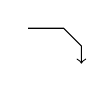
\begin{tikzpicture}[baseline=(O), scale=0.45]
		\coordinate (O) at (0, 0.5);
		\draw[->] (0, 1) -- (1, 1) -- (1.5, 0.5) -- (1.5, 0);
	\end{tikzpicture}$
	is $\identity_{X_1^*}$. This completes the proof.
\end{proof}

% segment-id: o014.aljabr2.chapter9.duality-a.p015
The relationship between left and right duals can be written as
${}^*(X^*)=X$ and $({}^*X)^*=X$. Although duality data are often chosen in
an argument or exposition, duality is fundamentally a property of an object,
not additional structure.

% segment-id: o014.aljabr2.chapter9.duality-a.ex001
\begin{example}
	In every monoidal category,
	% segment-id: o014.aljabr2.chapter9.duality-a.q005
	\[ \munit^* = \munit = {}^* \munit, \]
	and the required morphisms $\mathrm{ev}$ and $\mathrm{coev}$ both arise
	from the unit constraint $\munit\otimes\munit\simeq\munit$.
\end{example}

% segment-id: o014.aljabr2.chapter9.duality-a.d002
\begin{definition}[N.\ Saavedra Rivano]\label{def:rigid-cat}
	\index{monoidal category!rigid}
	If every object in a monoidal category $\mathcal{C}$ has a left dual
	(respectively, a right dual), then $\mathcal{C}$ is called a \emph{left
	rigid} (respectively, \emph{right rigid}) category.
\end{definition}

% segment-id: o014.aljabr2.chapter9.duality-a.p016
\index{string diagram}
The idea behind the proof of
Definition--Proposition~\ref{def:dual-uniqueness} is actually simple, but its
execution produces many formulas and commutative diagrams. In arguments
involving duality, a visualization technique called a \emph{string diagram}
is very useful; compare \S\ref{sec:alg-in-monoidal-cat} or
\cite[Proof of Theorem 2.6.12]{Li1}. More precisely, objects are drawn as
vertices and morphisms as arrows, with composition read from top to bottom.
For example, $\identity_X$, $f:X\to Y$, $g:Y\to Z$, and $gf$ are drawn,
respectively, as
% segment-id: o014.aljabr2.chapter9.duality-a.g007
\begin{center}\begin{tikzpicture}[morphism/.style={rectangle, draw, fill=white}]
		\node (A) {$X$};
		\node (B) [below=of A] {$X$};
		\path (A) edge (B);
		
		\node (X) [right=of A] {$X$};
		\node (Y) [below=of X] {$Y$};
		\path (X) edge[->] node[midway, morphism] {$f$} (Y);
		
		\node (Y2) [right=of X] {$Y$};
		\node (Z) [right=of Y] {$Z$};
		\path (Y2) edge[->] node[midway, morphism] {$g$} (Z);
		
		\node (X2) [right=of Y2] {$X$};
		\node (Z2) [below=2cm of X2] {$Z$};
		\path (X2) edge[->] node[near start, morphism] {$f$} node[near end, morphism] {$g$} (Z2);
\end{tikzpicture}\end{center}

% segment-id: o014.aljabr2.chapter9.duality-a.p017
Thus, pre- or postcomposing a morphism with $\identity$ amounts to extending
its arrow. The $\otimes$-product of morphisms is represented by placing
their arrows side by side; for example, $f\otimes g$ is drawn as
% segment-id: o014.aljabr2.chapter9.duality-a.g008
\begin{center}\begin{tikzpicture}[morphism/.style={rectangle, draw, fill=white}]
		\node (X) {$X$};
		\node (Y) [right=0.1cm of X] {$Y$};
		\node (Y1) [below=of X] {$Y$};
		\node (Z) [below=of Y] {$Z$};
		\path (X) edge[->] node[midway, morphism] {$f$} (Y1);
		\path (Y) edge[->] node[midway, morphism] {$g$} (Z);
\end{tikzpicture}\end{center}

% segment-id: o014.aljabr2.chapter9.duality-a.p018
Since $X\otimes\munit\simeq X\simeq\munit\otimes X$, the unit $\munit$
can be omitted from a string diagram; in other words, the string has no end
at that point. If the dual exists, the morphisms
$\mathrm{ev}:X\otimes X^*\to\munit$ and
$\mathrm{coev}:\munit\to X^*\otimes X$ are therefore drawn, respectively,
as
% segment-id: o014.aljabr2.chapter9.duality-a.g009
\begin{center}\begin{tikzpicture}[bend angle=70, auto]
		\node (L) {$X$};
		\node (R) [right=of L] {$X^*$};
		\path (L) edge[bend right] node[midway] {$\mathrm{ev}$} (R);
		
		\node (LL) [right=of R] {$X^*$};
		\node (RR) [right=of LL] {$X$};
		\path (LL) edge[bend left] node[midway] {$\mathrm{coev}$} (RR);
\end{tikzpicture}\end{center}

% segment-id: o014.aljabr2.chapter9.duality-a.p019
Under the same assumptions, the identities in
Definition~\ref{def:dualizable-obj},
% segment-id: o014.aljabr2.chapter9.duality-a.q006
\[ (\identity_X \otimes \mathrm{ev}) (\mathrm{coev} \otimes \identity_X ) = \identity_X = (\mathrm{ev} \otimes \identity_X) (\identity_X \otimes \mathrm{coev}) \]
are represented by
% segment-id: o014.aljabr2.chapter9.duality-a.e001
\begin{equation}\label{eqn:Zorro}
	\begin{tikzpicture}[baseline=(B), bend angle=70, auto]
		\node (A) {$X$};
		\node (B) [below=of A] {$X$};
		\node (C) [left=of B] {${}^* X$};
		\node (D) [left=of C] {$X$};
		\node (E) [below=of D] {$X$};
		
		\path (A) edge (B);
		\path (D) edge[bend left] node {$\mathrm{coev}$} (C);
		\path (C) edge[bend right] node {$\mathrm{ev}$} (B);
		
		\path (D) edge[->] (E);
	\end{tikzpicture} \quad = \quad
	\begin{tikzpicture}[baseline=(M)]
		\node (A) {$X$};
		\node (M) [below=of A] {};
		\node (B) [below=of M] {$X$};
		\path (A) edge (B);
		\coordinate (M) at ($(A)!.5!(B)$);
	\end{tikzpicture} \quad = \quad
	\begin{tikzpicture}[baseline=(B), bend angle=70, auto]
		\node (A) {$X$};
		\node (B) [below=of A] {$X$};
		\node (C) [right=of B] {$X^*$};
		\node (D) [right=of C] {$X$};
		\node (E) [below=of D] {$X$};
		
		\path (A) edge (B);
		\path (C) edge[bend left] node {$\mathrm{coev}$} (D);
		\path (B) edge[bend right] node {$\mathrm{ev}$} (C);
		
		\path (D) edge[->] (E);
	\end{tikzpicture}
\end{equation}
provided, of course, that the duals in question exist. These diagrams give
Definition~\ref{def:dualizable-obj} the operational flavor of ``straightening
a string.'' In some of the literature, the diagrams above are drawn after a
rotation by $\frac{\pi}{2}$ and are therefore also called the \emph{Z
identities}.
\index{Z identity (mark of Zorro)}

% segment-id: o014.aljabr2.chapter9.duality-a.p020
By the correspondence between algebraic identities and operations on string
diagrams, basic algebraic identities involving duality can be found simply
by following the diagrams, or even proved directly from them. As an
exercise, the reader may try to rewrite the proof of
Definition--Proposition~\ref{def:dual-uniqueness} as a simple diagram.

% segment-id: o014.aljabr2.chapter9.duality-a.p021
The following result shows that duality naturally reverses the order of
$\otimes$.

% segment-id: o014.aljabr2.chapter9.duality-a.pr002
\begin{proposition}
	Let $\mathcal{C}$ be a monoidal category and
	$X,Y\in\Obj(\mathcal{C})$.
	\begin{enumerate}[(i)]
		% segment-id: o014.aljabr2.chapter9.duality-a.i003
		\item If $X$ and $Y$ have left duals ${}^*X$ and ${}^*Y$,
		respectively, then ${}^*Y\otimes{}^*X$ is a left dual of $X\otimes Y$.
		The corresponding data can be depicted in terms of the duality data of
		$X$ and $Y$ as
		% segment-id: o014.aljabr2.chapter9.duality-a.e002
		\begin{equation*}
			\mathrm{ev}_{X \otimes Y} = \left[ \begin{tikzcd}[column sep=tiny, ampersand replacement=\&]
				{}^* Y \arrow[dash, rrr, bend right=80, "{\mathrm{ev}_Y}"' near end] \& {}^* X \arrow[dash, r, bend right=60, "{\mathrm{ev}_X}"' near start] \& X \& Y
			\end{tikzcd}\right], \quad
			\mathrm{coev}_{X \otimes Y} = \left[ \begin{tikzcd}[column sep=tiny, ampersand replacement=\&]
				X \arrow[dash, rrr, bend left=80, "{\mathrm{coev}_X}" near start] \& Y \arrow[dash, r, bend left=60, "{\mathrm{coev}_Y}" near end] \& {}^* Y \& {}^* X
			\end{tikzcd}\right].
		\end{equation*}
		% segment-id: o014.aljabr2.chapter9.duality-a.i004
		\item If $X$ and $Y$ have right duals $X^*$ and $Y^*$,
		respectively, then $Y^*\otimes X^*$ is a right dual of $X\otimes Y$.
		The corresponding data can be depicted in terms of the duality data of
		$X$ and $Y$ as
		% segment-id: o014.aljabr2.chapter9.duality-a.e003
		\begin{equation*}
			\mathrm{ev}_{X \otimes Y} = \left[ \begin{tikzcd}[column sep=tiny, ampersand replacement=\&]
				X \arrow[dash, rrr, bend right=80, "{\mathrm{ev}_X}"' near end] \& Y \arrow[dash, r, bend right=60, "{\mathrm{ev}_Y}"' near start] \& Y^* \& X^*
			\end{tikzcd}\right], \quad
			\mathrm{coev}_{X \otimes Y} = \left[ \begin{tikzcd}[column sep=tiny, ampersand replacement=\&]
				X^* \arrow[dash, rrr, bend left=80, "{\mathrm{coev}_X}" near end] \& Y^* \arrow[dash, r, bend left=60, "{\mathrm{coev}_Y}" near start] \& Y \& X
			\end{tikzcd}\right].
		\end{equation*}
	\end{enumerate}
\end{proposition}
% segment-id: o014.aljabr2.chapter9.duality-a.pf003
\begin{proof}
	We must verify the identities in
	Definition~\ref{def:dualizable-obj}, namely the Z identities
	\eqref{eqn:Zorro}. Equivalently, we must check that
	% segment-id: o014.aljabr2.chapter9.duality-a.q007
	\begin{align*}
		\begin{tikzcd}[column sep=tiny, ampersand replacement=\&]
			{}^* Y \arrow[dash, rrr, bend right=80] \& {}^* X \arrow[dash, r, bend right=60] \& X \arrow[dash, rrr, bend left=80] \& Y \arrow[dash, r, bend left=60] \& {}^* Y \& {}^* X
		\end{tikzcd} & = \begin{tikzcd}[column sep=tiny, ampersand replacement=\&]
			{}^* Y \arrow[dash, d] \& {}^* X \arrow[dash, d] \\
			{}^* Y \& {}^* X 
		\end{tikzcd}, \\
		\begin{tikzcd}[column sep=tiny, ampersand replacement=\&]
			X \arrow[dash, rrr, bend left=80] \& Y \arrow[dash, r, bend left=60] \& {}^* Y \arrow[dash, rrr, bend right=80] \& {}^* X \arrow[dash, r, bend right=60] \& X \& Y
		\end{tikzcd} & = \begin{tikzcd}[column sep=tiny, ampersand replacement=\&]
			X \arrow[dash, d] \& Y \arrow[dash, d] \\
			X \& Y 
		\end{tikzcd}
	\end{align*}
	Strictly speaking, the diagrams on the left should be stretched in the
	vertical direction as in \eqref{eqn:Zorro}: insert several copies of
	$\identity$, shift them horizontally as appropriate, and then straighten
	them. The identities above are then clear. The corresponding formal
	verification is based on the various naturality properties of the unit
	constraints; the details are left to the interested reader.
\end{proof}

% segment-id: o014.aljabr2.chapter9.duality-a.d003
\begin{definition}\label{def:dual-morphism}
	\index[sym1]{f-star@$f^*, {}^* f$}
	Let $f:X\to Y$ be a morphism in a monoidal category $\mathcal{C}$.
	Suppose that $X$ and $Y$ both have left duals ${}^*X$ and ${}^*Y$
	(respectively, right duals $X^*$ and $Y^*$). The left dual morphism
	${}^*f:{}^*Y\to{}^*X$ (respectively, the right dual morphism
	$f^*:Y^*\to X^*$) of $f$ is defined as follows:
	% segment-id: o014.aljabr2.chapter9.duality-a.e004
	\begin{equation*}\begin{aligned}
		% segment-id: o014.aljabr2.chapter9.duality-a.q008
		{}^* f := (\mathrm{ev}_Y \otimes \identity) (\identity \otimes f \otimes \identity) (\identity \otimes \mathrm{coev}_X) \; &
		\begin{tikzpicture}[baseline=(T), bend angle=70, auto]
			\node (A) {${}^* Y$};
			\node (B) [below=of A] {${}^* Y$};
			\node (C) [right=of B] {$Y$};
			\node (S) [right=of A] {$X$};
			\node[draw, fill=white] (T) at ($(S)!.5!(C)$) {$f$};
			\node (D) [right=of S] {${}^* X$}; 
			\node (E) [below=of D] {${}^* X$};
				
			\path (A) edge (B);
			\path (B) edge[bend right] node {$\mathrm{ev}_Y$} (C);
			\path (C) edge (T);
			\path (T) edge (S);
			\path (S) edge[bend left] node {$\mathrm{coev}_X$} (D);
			\path (D) edge[->] (E);
		\end{tikzpicture}, \\
		% segment-id: o014.aljabr2.chapter9.duality-a.q009
		f^* := (\identity \otimes \mathrm{ev}_Y) (\identity \otimes f \otimes \identity) (\mathrm{coev}_X \otimes \identity) \; &
		\begin{tikzpicture}[baseline=(T), bend angle=70, auto]
			\node (A) {$Y^*$};
			\node (B) [below=of A] {$Y^*$};
			\node (C) [left=of B] {$Y$};
			\node (S) [left=of A] {$X$};
			\node[draw, fill=white] (T) at ($(S)!.5!(C)$) {$f$};
			\node (D) [left=of S] {$X^*$}; 
			\node (E) [below=of D] {$X^*$};
				
			\path (A) edge (B);
			\path (C) edge[bend right] node {$\mathrm{ev}_Y$} (B);
			\path (C) edge (T);
			\path (T) edge (S);
			\path (D) edge[bend left] node {$\mathrm{coev}_X$} (S);
			\path (D) edge[->] (E);
		\end{tikzpicture}.
	\end{aligned}\end{equation*}
\end{definition}
